\documentclass[a4paper, 12pt, UTF8]{article}

\usepackage[dvipsnames]{xcolor} % Code highlighting color
\usepackage[spanish]{babel} % Language 
\usepackage{indentfirst}
\usepackage{fontspec} 
\usepackage{fullpage}
\usepackage{csquotes}
\usepackage[a4paper, margin=2cm]{geometry} % To change the margins
\usepackage{graphicx} % Insert images
\usepackage[hidelinks]{hyperref} % Links color
\usepackage[final]{pdfpages}
\usepackage{ragged2e}
\usepackage{wrapfig} %To Text wrap
\usepackage{listings} % Add code
\usepackage{verbatim}
\usepackage[backend=bibtex,citestyle=ieee]{biblatex}
\usepackage{nameref}
\usepackage{tikz}
\usepackage{float}
\usepackage{subcaption}
\usepackage{url}
\usepackage{multirow}
\usepackage{colortbl}

\setlength{\parskip}{0.7em}
%\setlength{\parindent}{1cm}
\linespread{1.2}

\title{
	\Huge
	\textbf{Trabajo innovación} \\
	\scshape Uso de redes neuronales para la clasificación de células
	}
\author{
	Marc Asenjo i Ponce de León \and
	Joan Marcè i Igual \and
	Iñigo Moreno i Caireta
	}
\date{\today}

\addbibresource{Bibliografia.bib}


\begin{document}

\maketitle

\begin{figure}
	\centering
	
\includegraphics[width=\linewidth]{./simple_FIB}
\end{figure}

\newpage
\tableofcontents

\newpage

\section{Introducción}

En este trabajo nos hemos centrado en la investigación\cite{deepLearning} sobre distintos métodos de clasificación de células y como las redes neuronales pueden afectar a dichos métodos.

\section{Impacto del descubrimiento}

Esta investigación permite hacer operaciones más profundas ya que normalmente el impacto que puede ocasionar la clasificación clásica puede generar que se activen o se inhiban ciertas señales, cambiando el comportamiento de ciertos tipos de células. Así pues este estudio permite sobrepasar estos problemas ya que no es necesario marcar las células para investigarlas y se puede hacer con una gran precisión y velocidad.

Como con este análisis se puede obtener más precisión, sensibilidad y seguridad, se está empezando a trabajar en la clasificación de células en busca de las que son potencialmente cancerígenas. En la \hyperref[fig:impacto_1]{Figura~\ref{fig:impacto_1}} se observa como este tipo de análisis permite obtener todo un conjunto de características para cada célula individualmente. 
Así pues, es relativamente fácil, a partir de ciertos parámetros, adivinar si hay células cancerígenas dentro del organismo y saber cuáles son.

\begin{figure}[H]
	\centering
	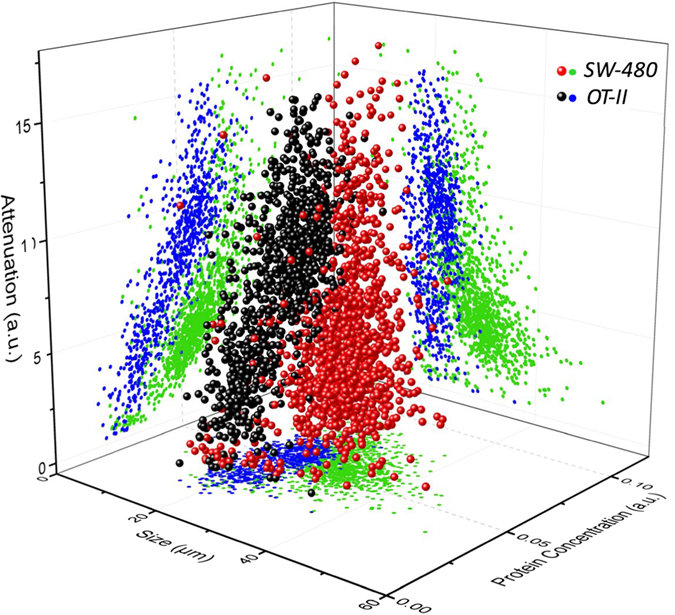
\includegraphics[width=0.95\textwidth]{impacto_1}
	\caption{Ejemplo de la clasificación de células cancerígenas donde se han ordenado en función de su tamaño, concentración de proteínas y atenuación}
	\label{fig:impacto_1}
\end{figure}

Otro ejemplo de uso son los biofueles generados a partir de microorganismos. Estos convierten el dióxido de carbono en lípidos que son mejores que los obtenidos por la agricultura tradicional. 

Actualmente, en todo el mundo se esta intentando mejorar la productividad de estos microorganismos y con este método podrán ser capaces de seleccionar directamente las micro algas que tienen un factor de crecimiento mayor y esto, es esencial en la industria de producción de biofuel para poder generar grandes cantidades de este producto y rebajar los costes. Se puede ver en la \hyperref[fig:impacto_2]{Figura \ref{fig:impacto_2}} como se han podido clasificar las diferentes algas en función de los contenidos de lípidos.

\begin{figure}[H]
	\centering
	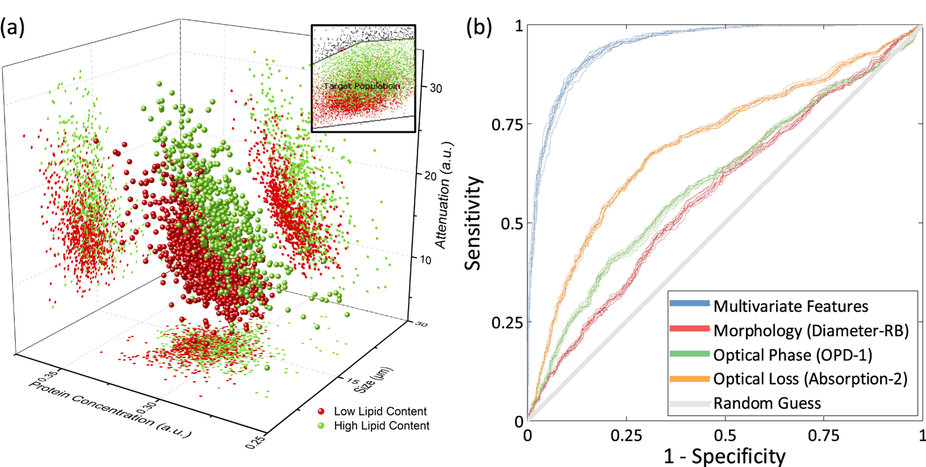
\includegraphics[width=\linewidth]{impacto_2}
	\caption{Ejemplo de la clasificación de micro algas, separando las que tienen un alto contenido de lípidos de las que tienen uno bajo}
	\label{fig:impacto_2}
\end{figure}

Así pues se puede ver que con este sistema se obtiene muchísima más precisión que con los métodos anteriores de manera que abre las puertas a un nuevo campo donde cada microorganismo se pueda clasificar individualmente. Se esta empezando a trabajar también en los microbots \cite{microbots} y quizá en un futuro se puedan emplear para clasificar todo aquello que no debería estar dentro de nuestro organismo como por ejemplo las bacterias o toda esa grasa innecesaria. 

\printbibliography

\end{document}